\chapter{Project Plan}
    This chapter will briefly talk about the 5S Drifter project motivations as well their function as a product developed 
    by the Minho's University under supervision by the professors Luis Gonçalves and Sérgio Lopes.
\section{Introduction}
Under the course unity of Integrative Project in Industrial Electronics and Computers the students must
apply for professors projects in order to integrate unde their respective laboratories and start to undertand the pace
demanded on the Master's final paper.

This project, given by the professor Luis Gonçalves and Sergio Lopes under the CMEMS laboratory,
has the main porpouse to create a drifter for data aquisition. As a multi-themed project, this report will
explore multiple areas, as the PCB design for hardware and firmware manufacture, software design under the idea to optimize
the execution allowing for better performance. The main goal is to have the final product afloat at the end of the simester.

\subsection{Problem Statement}
The ocean is one of the man greatest mistery even before the written history. Humanity made the world ours over the water, 
from the Portuguese greatests discoveries, braving the raging ocean to the newst oil tanker demanding ever newer technology
in order to tame the sea for safer and smother sailing.

Nowadays cientists belive only 5\% of the ocean is discovered with the actual technology witch means that humanity 
know as much about our so grate sky as our own seas. 5S ocean drifter is a equipament made to acquire date from 
superficial sea streams and expand the oceangrapgh knowledge about it.

Better knowledge of the ocean lead to further development in diverse areas. Granting safety,
security and efficiency.

5S, an acronym for Sensoring System for Surface Sea Streams is a lowcost, lowpower solution to acquire
said data with the focus to last autonomously for the longest time possible. The drifter has to attain its GPS
coordenates in order to track its current and avarege velocity, alongside with the water temperature and a accelerometer 
information to gether information about the wave intencity. All this data will be transmitted by a protocol,
 yet to be defined, with a JASON format in order to be read by a database that allready is implemented.  


\subsubsection{Transport}
Sadly, it isn't uncommon to see transport accidents being reported, and even worse, for it to be a gigantic problem.
Some of these accidents are caused by poor mapping of sea conditions, tankers spilling oil, fishing vessels capsizing, leading
to financial problems and even loss of life. Even when there are no accidents, poor knowledge of tides results in higher energy consumption when routes are set against the currents.

A solution would be to create optimized shipping routes, minimizing accidents and improving energy efficiency while 
traversing the waves. Oil tankers could follow currents with lower fuel consumption. Fishing routes could become more
efficient, as their target species may swim with the tides based on temperature and speed. This would ease the workload,
making the activity less reactive and more predictable, aligning expected catch rates with reduced time and energy 
consumption.

A well-known example of a hazardous area is the Nazaré Canyon, where its unique shape creates enormous waves. 
Avoiding these waters is crucial for safer navigation.

\subsubsection{Ecology}


Habitats 

The placement of wave energy converters, a growing field under the energy generation, is one of the main problems the
technology faces. A good positioning improves the efficiency
\begin{center}
    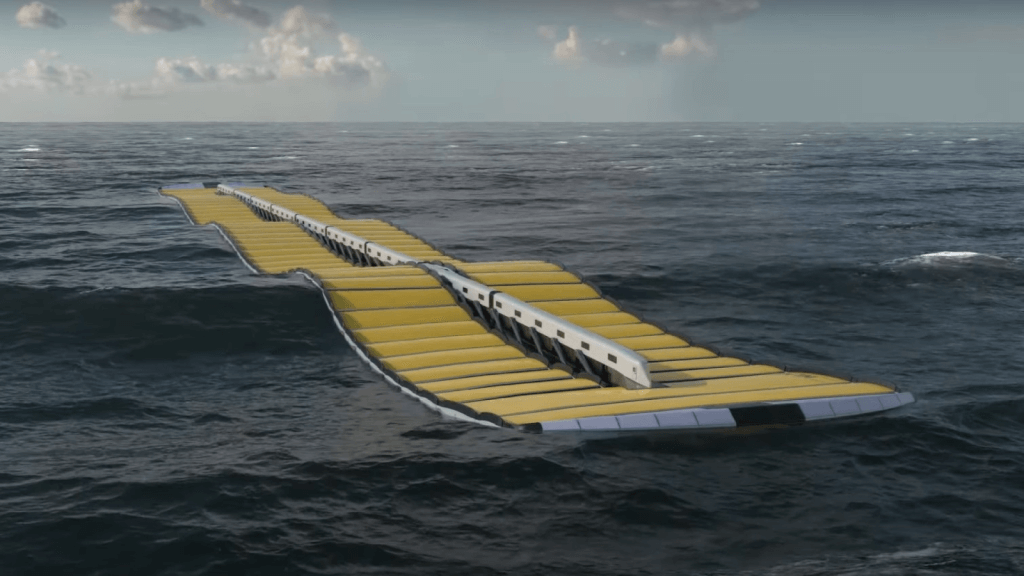
\includegraphics[width=0.7\textwidth]{images/chapter/introduction/renewable_energy.png}  % Adjust the width as necessary
    %\caption{This is a Header_image}
    \label{fig:The Design of a Wave Energy Converter to Electricity}        
\end{center}

Renewable Energy 

\subsubsection{Oceanograpy}
Better undertanding of the Iberian Poleward Current (IPC)

\subsubsection{Geology}

Know where the sedimentation is leading to
\subsubsection{Sports}

\subsection{Problem Statement Analysis}

waterfall

vila do conde + ou - 10km mar adentro 2g 4g\\
mapa de alcance na costa\\
atenção ao clima \\
latencia / sampling / tamanho do cartão sd\\ 
autonomia de NO MINIMO 50 DIAS \\
consumo médio max 5mA \\
distancia da antena e da água \\
IMU caso tenha espaço para o consumo \\
SD memoria local \\
ADC a bateria \\
sensor de temperatura \\
database mongo db \\
